\chapter{Method details}
This chapter presents additional details on the experimental work performed as part of this thesis. It builds directly on the material presented in the article, which describes only the most relevant and critical details. Additional results and experiments are presented in the next chapter.

The primary contribution of this work in terms of implemented software, is the platform designed and created for the experimental work presented in the article. The platform consists of tools for optimisation, entropy calculations, iris recognition, gaze estimation as well as a platform for defining, running, and analysing iris obfuscation experiments. 


\section{Implementation details}
This section presents the scope and important details of the software systems implemented for the thesis. One of the goals of the thesis is to create an experimental platform that can easily be extended and adapted for future research.

FIGREF shows a high-level diagram of the provided software. 

T


\subsection{Optimisation engine}\label{sec:detail-opt}
The parameter experiments presented in the article are driven by the optimisation engine component. Its purpose is to allow implementation of a number of different optimisation methods.

The MultiObjectiveOptimizer class expects an Objective and produces a set of results by calling its run method. The run method is implemented differently for each subclass to support different types of optimisation. The NaiveMultiObjectiveOptimizer does not use feedback for determining parameters for the next iteration and instead relies on sampling based parameter selection - this is the class used in the experiments. Additionally, a PopulationMultiObjectiveOptimizer is an implementation of the so called \textit{vector evaluated genetic algorithm} \parencite{kochenderfer2019algorithms}, which uses population strategies to combine and select parameters. The method is discussed in further detail in \cref{sec:future-optim}, where its possible uses for future work is considered.

Each optimiser has exactly one Objective. The abstract Objective class only has a single sub-class ObfuscationObjective for now but additional ones would be necessary for other optimisation methods or other optimisation tasks. The purpose of the Objective class is to calculate a set of Metrics given a set of parameters. In ObfuscationObjective this is done as described in the article by using different datasets for different metrics. 

Specifically, the objective object is initialised with a pool of datasets divided into three categories: Iris datasets, Gaze datasets, and pupil centre datasets. As seen on the class diagram, this terminology arises from the fact that the gaze datasets are subdivided. The objective can be initialised with any number of different metrics provided as objects. Calling the \emph{eval} function results in the metrics being calculated for a number of samples drawn from the datasets. The sample size is determined at the moment of initialisation.

Results are recorded in a special Logger object, which wraps a dictionary and provides convenient methods for accessing the data. In terms of the optimisation experiment described in the article, each obfuscation method represents one MultiObjectiveOptimizer instance.

\subsection{Experiment platform and interactive tools}
\begin{figure}
	\begin{subfigure}{0.3\textwidth}\centering
		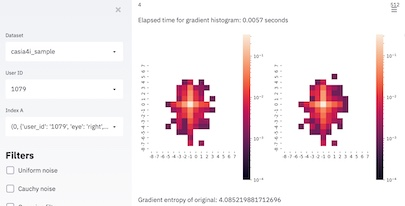
\includegraphics[width=1\linewidth]{figures/labs/EntropyLab}
		\caption{Entropylab}\label{fig:tools:entropylab}
	\end{subfigure}
	\hfill
	\begin{subfigure}{0.3\textwidth}\centering
		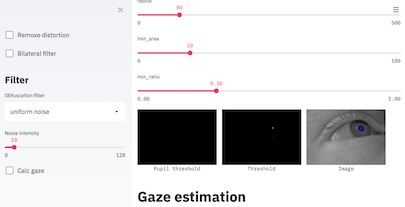
\includegraphics[width=1\linewidth]{figures/labs/GazeLab}
		\caption{GazeLab}\label{fig:tools:gazelab}
	\end{subfigure}
	\hfill
	\begin{subfigure}{0.3\textwidth}\centering
		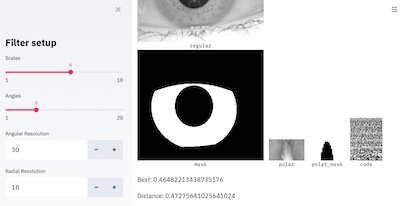
\includegraphics[width=1\linewidth]{figures/labs/ObfuscationLab}
		\caption{ObfuscationLab}\label{fig:tools:obfuscationlab}
	\end{subfigure}
	\\
	\begin{subfigure}{0.3\textwidth}\centering
		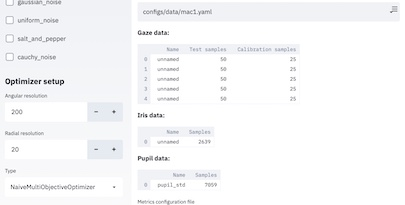
\includegraphics[width=1\linewidth]{figures/labs/OptimisationLab}
		\caption{OptimisationLab}\label{fig:tools:optimisationlab}
	\end{subfigure}
	\hfill
	\begin{subfigure}{0.3\textwidth}\centering
		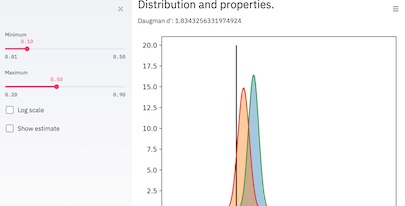
\includegraphics[width=1\linewidth]{figures/labs/ObfuscationResultAnalyser}
		\caption{ObfuscationResultAnalyser}\label{fig:tools:obfuscationresultanalyser}
	\end{subfigure}
	\hfill
	\begin{subfigure}{0.3\textwidth}\centering
		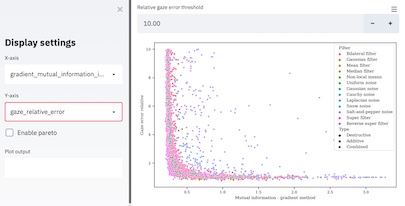
\includegraphics[width=1\linewidth]{figures/labs/OptimisationResultAnalyser}
		\caption{OptimisationResultAnalyser}\label{fig:tools:optimisationresultanalyser}
	\end{subfigure}
	
	\caption{Screenshots showing the individual interactive tools. The code is, of course, included with the thesis submission as well.}\label{fig:tools}
\end{figure}

The experimental platform is bound together by a number of data-formats describing the precise configurations used for each experiment. This allows easy reproducibility and comparison between methods. The configuration files are modified either manually or by using one of the six interactive tools developed for experimentation and result analysis. 

The interactive tools are either self-contained and created for experimentation with the approaches used or they are meant as configuration and analysis tools for experimentation.

Six different interactive tools were created, specifically
\begin{description}
	\item [EntropyLab] Tool for experimenting with image-based entropy measurements and their distributions.
	\item [GazeLab] Tool for experimenting with gaze estimation parameters and evaluating performance.
	\item [ObfuscationLab] Explorative tool for testing the iris obfuscation algorithm and setting up configuration files for large-scale testing. 
	\item [OptimisationLab] Tool used for running small optimisation experiments and creating configurations for larger ones. 
	\item [ObfuscationResultsAnalyser] For testing the result of running the iris obfuscation experiment. Only allows simple analyses and was mostly used during development of the iris recognition algorithm to test performance.
	\item [OptimisationResultsAnalyser] Detailed interactive analysis for the parameter experiments. It has been used primarily to discover interesting facets of the results. Due to the large number of metrics used for analysis, interactive visualisations provide....
\end{description}


\section{Gaze estimation}
For this project, I chose to implement my own gaze estimation system. Although previous students at ITU have developed eye tracking software which was available to me, both the system and the hardware was not ideal for this use case either. 

The physical setup is a remote camera that is positioned close to the eye to create circumstances similar to head-mounted eye trackers. Participants are asked to rest their head on a stand which ensures relative stability of the eye's location relative to the camera. A screen is used to show target which are to be predicted by the software. An infrared LED fastened to the screen acts as both a light and for creating a corneal reflection. Details on calibration are left to the article.

To estimate the gaze point from any given image, the system uses a pupil-glint vector as a source which is then mapped from image to screen coordinates using a two-dimensional polynomial. The glint effectively acts as an origin for the system since it is stationary. The coefficients of the polynomial are found using the least-squares method on a set of calibration points where the target screen position is known.

For a set of pupil-glint vectors $\{\mathbf{x}^1, \mathbf{x}^2, \dots, \mathbf{x}^n\}$ and corresponding screen positions $\{\mathbf{y}^1, \mathbf{y}^2, \dots, \mathbf{y}^n\}$, a second-degree model requires two functions of both input variables which can be written
\begin{equation}
    \mathbf{y}^i =  \begin{bmatrix}
        \left(x_1^{1}\right)^2 & \left(x_2^{1}\right)^2 & x_1^1x_2^1 x_1^1 & x_2^1 & 1\end{bmatrix} \begin{bmatrix}a^1&a^2\\ b^1&b^2\\ c^1&c^2\\ d^1&d^2\\ e^1&e^2\\ f^1&f^2\end{bmatrix},
\end{equation}
where $a$-$e$ are the parameters. A solution could be found using $12$ calibration points, but the method of least squares allows us to minimise the impact of outliers.

Several pupil detectors were tested, of which DeepEye \parencite{vera2019deepeye} outperformed the others. Specifically, I tested a home-made BLOB based detector and the ElSE \parencite{fuhl2016else} and ExCuSE \parencite{excuse} detectors as well.

\subsection{Iris recognition}


%Compared to similar implementations, it compares similarly, with an equal error rate of $xx$. Daugman's original implementation 


%The iris recognition implementation is an attempt at closely matching the design of the original algorithm created by Daugman (REF) and which is generally still used for baseline comparisons today. In improved versions, Daugman's method acheives accuracies of XX on a non-public dataset. The replica only achieves XX on the CASIA IV dataset though it should be mentioned that this is very favourable compared to other replicas proposed in various studies (REF). Additionally the test dataset, CASIA IV, only contains $2639$ samples from $xx$ subjects which limits the precision of the result.

The iris implementation used in the experiments has been implemented from scratch. There are two reasons for this choice. By far the most important was that no accurate implementation was available with support for Python. The source code for the OSIRIS project \parencite{osiris} has seemingly disappeared and several others including \parencite{rec1, rec2, rec3} did not use the original technique. Secondly, implementing the method from scratch provides valuable experience which is useful when trying to understand how the iris signal is communicated and decoded from its image representation.

% A very thorough implementation of multiple iris recognition algorithms are available in a library (REF) but only in c++. Writing a Python interface was outside the scope of this thesis.


Daugman's method is based on the use of wavelets to detect the phase of the iris at a number of frequencies and angles. The minimum wavelength chosen for the filters was 3 pixels in order to avoid artefacts affecting the outcome. This minimum is limited by the Nyquist frequency\todo{check this}

\begin{figure}
    \begin{subfigure}{0.5\linewidth}
        \centering
        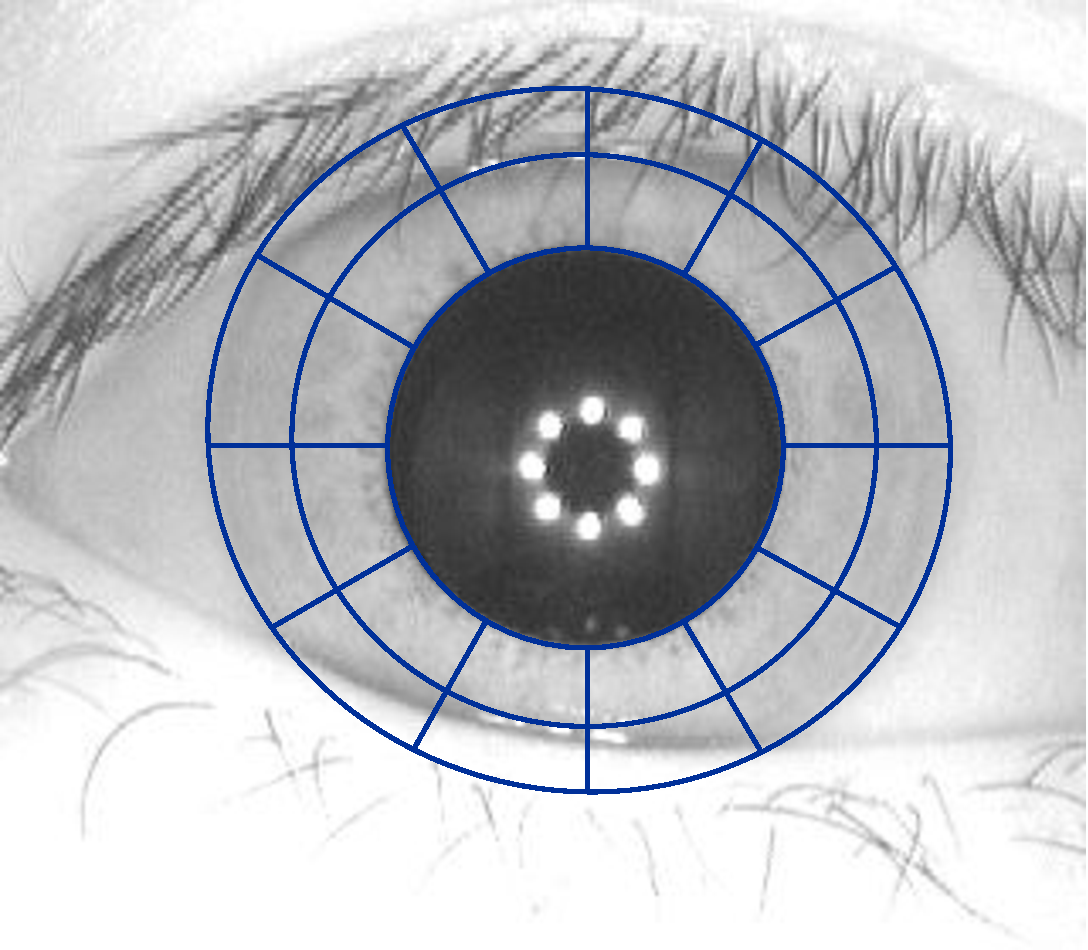
\includegraphics[width=0.6\linewidth]{figures/polar-image.pdf}
        \caption{The pupil and iris circumference ellipses define a polar coordinate system.}
        \label{fig:polar-method-a}
    \end{subfigure}
    \begin{subfigure}{0.5\linewidth}
        \centering
        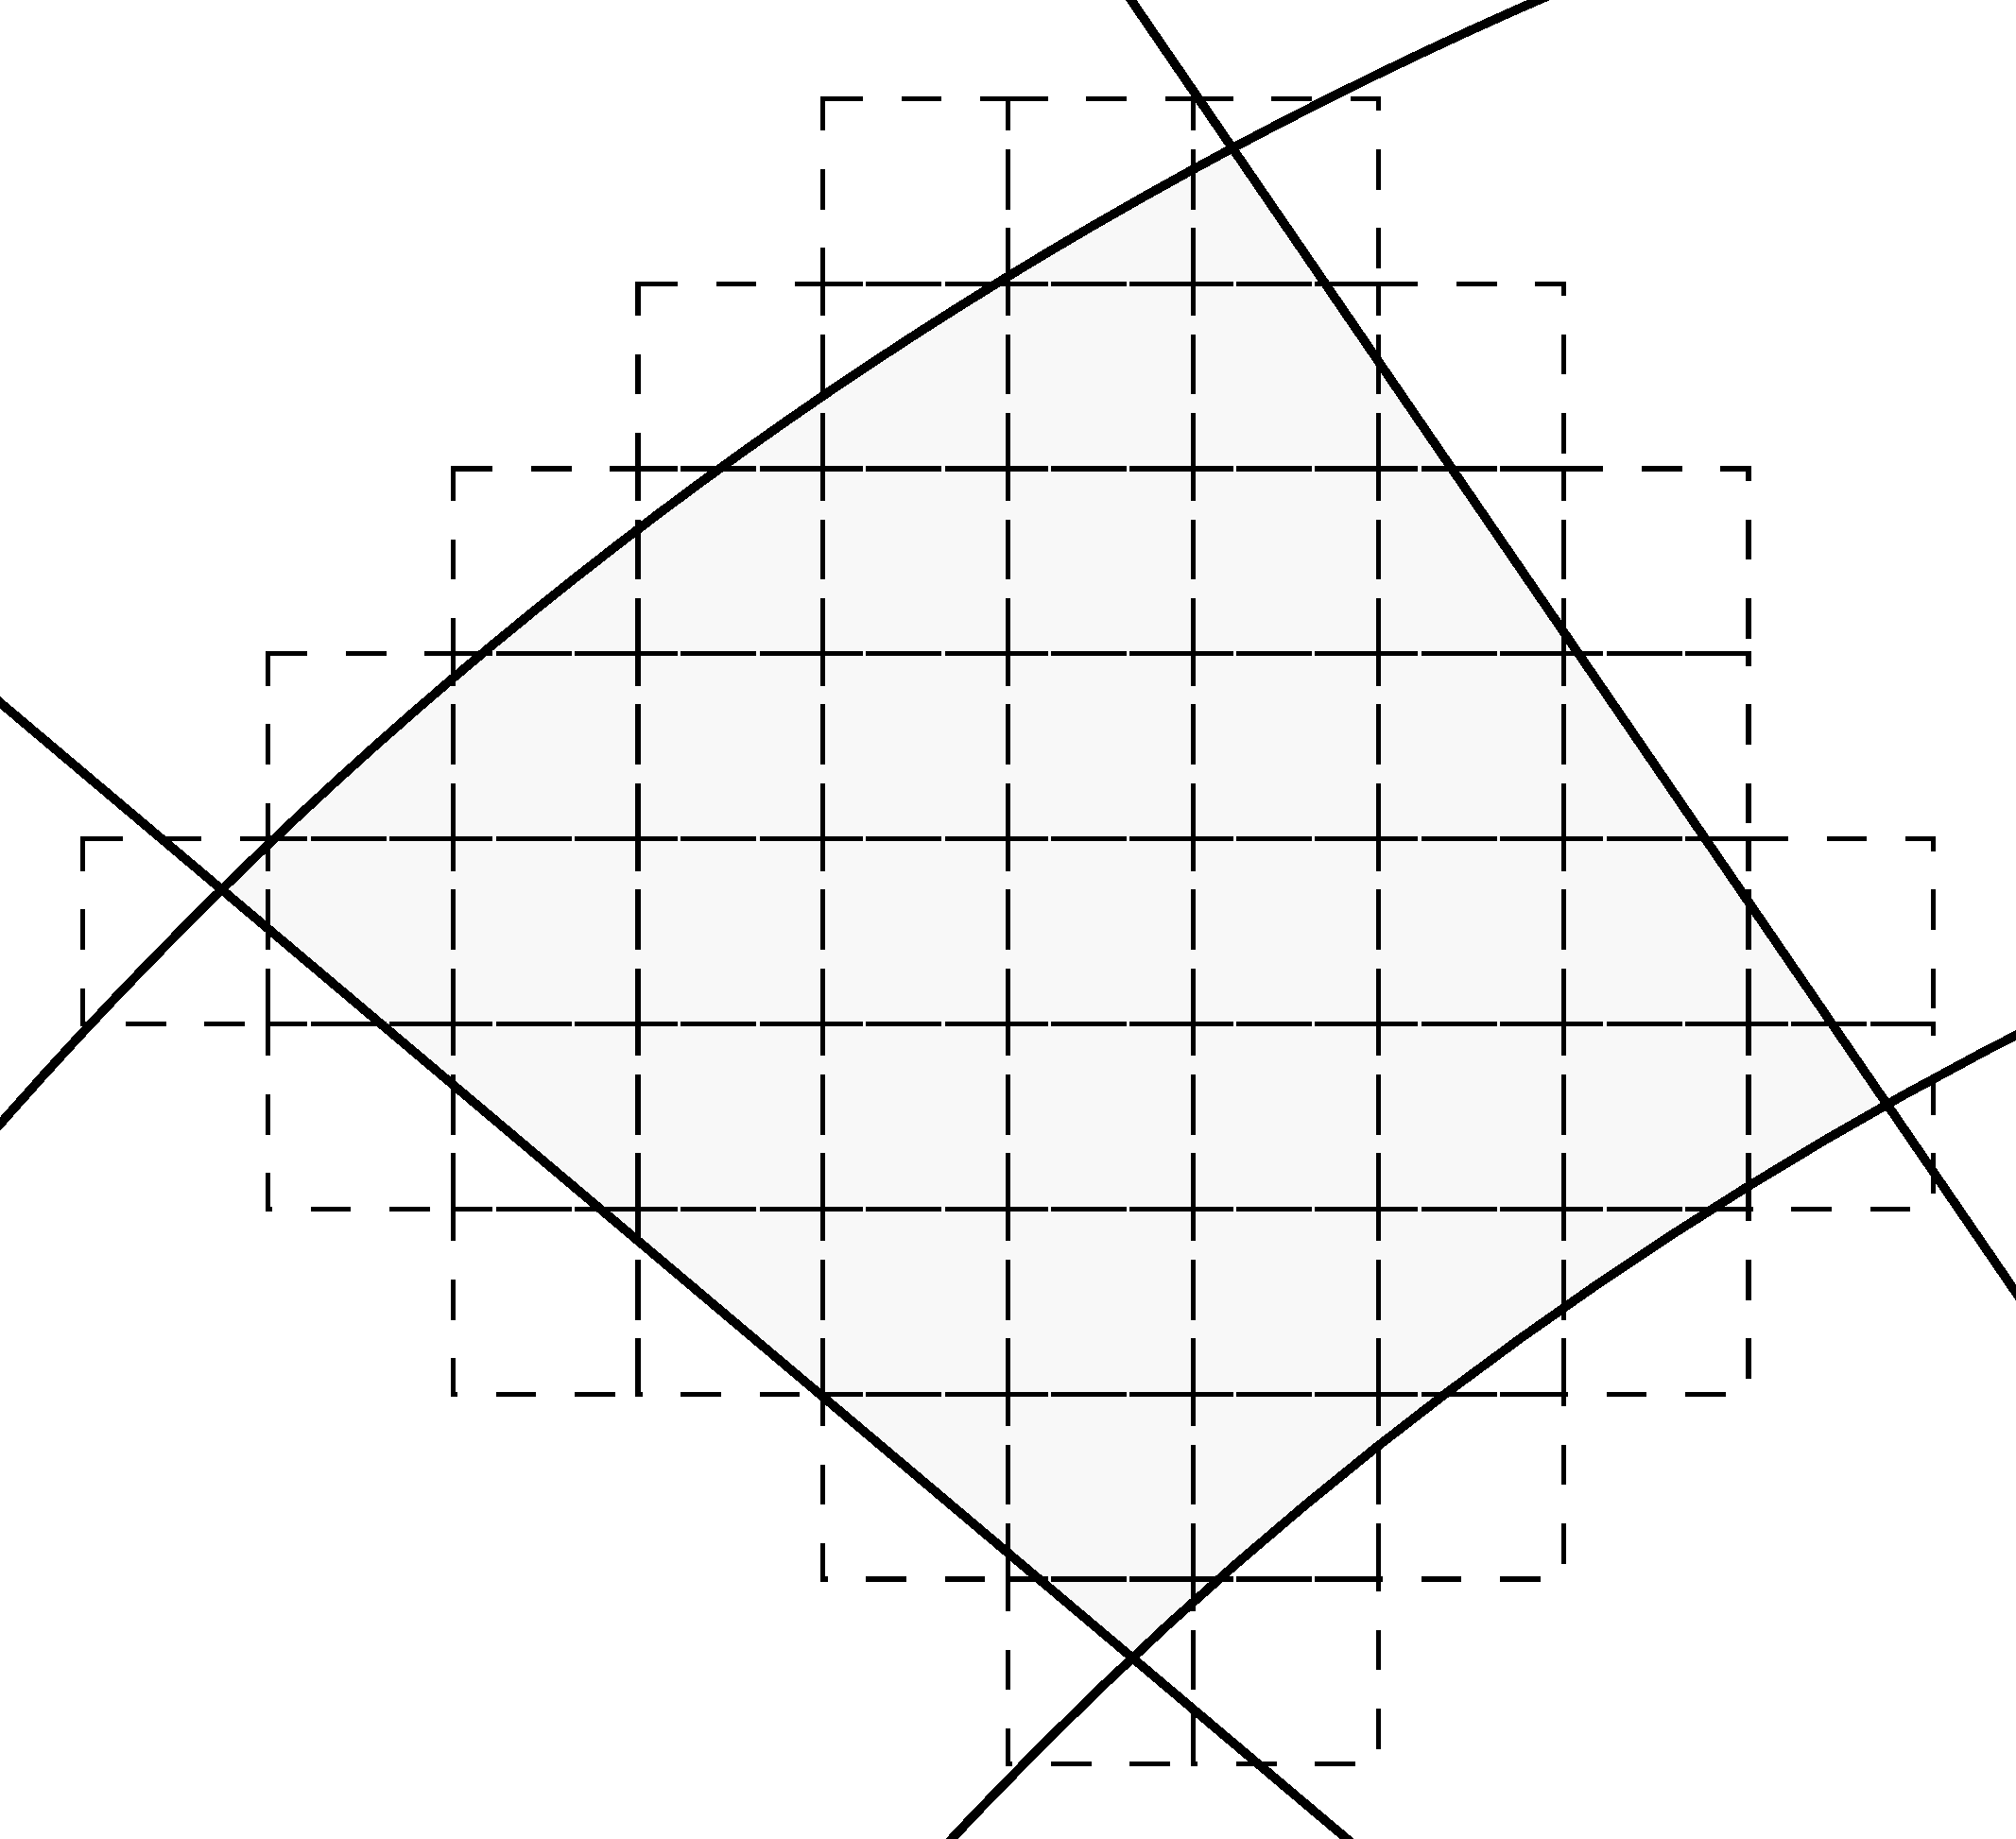
\includegraphics[width=0.6\linewidth]{figures/polar-method.pdf}
        \caption{Individual pixels in the polar coordinate system covers many actual pixels in the original cartesian space. The effect is amplified in the figure.}
        \label{fig:polar-method-b}
    \end{subfigure}
    \caption{}\label{fig:polar-method}
\end{figure}

The polar sampling method uses a particularly interesting technique. As shown in \cref{fig:polar-method}, the pseudo-polar coordinate system results in pixels that overlap several of the original image's pixels in strange ways. A possible solution would be to radically increase the polar resolution and use bilinear sampling or similar for interpolation. 

Due to the relatively slow phase calculation implementation however, I chose to keep the polar resolution low and instead opted to use a simple probabilistic sampling technique. If we denote the polar pixel region as a set $S$, each pixel in the cartesian image coordinate system is similarly sets $C_1, \dots, C_n$. The ideal pixel value at that coordinate is then:
\begin{equation}
    P(S) = \frac{\sum_{i=1}^n I_i A(S\cap C_i)}{A(S)}
\end{equation}

In other words, the pixel should take on the average value of the underlying pixels weighted by their intersecting areas. An easy way to implement this is by randomly sampling points inside $S$, adding their values, and dividing by $n$
\begin{equation}
    P(S) = \frac{1}{n}\sum_{x \sim U(S)}^n I_{x},
\end{equation}
where $U(S)$ is a uniform distribution over $S$. This method works for any size...

\begin{figure}
    \centering
    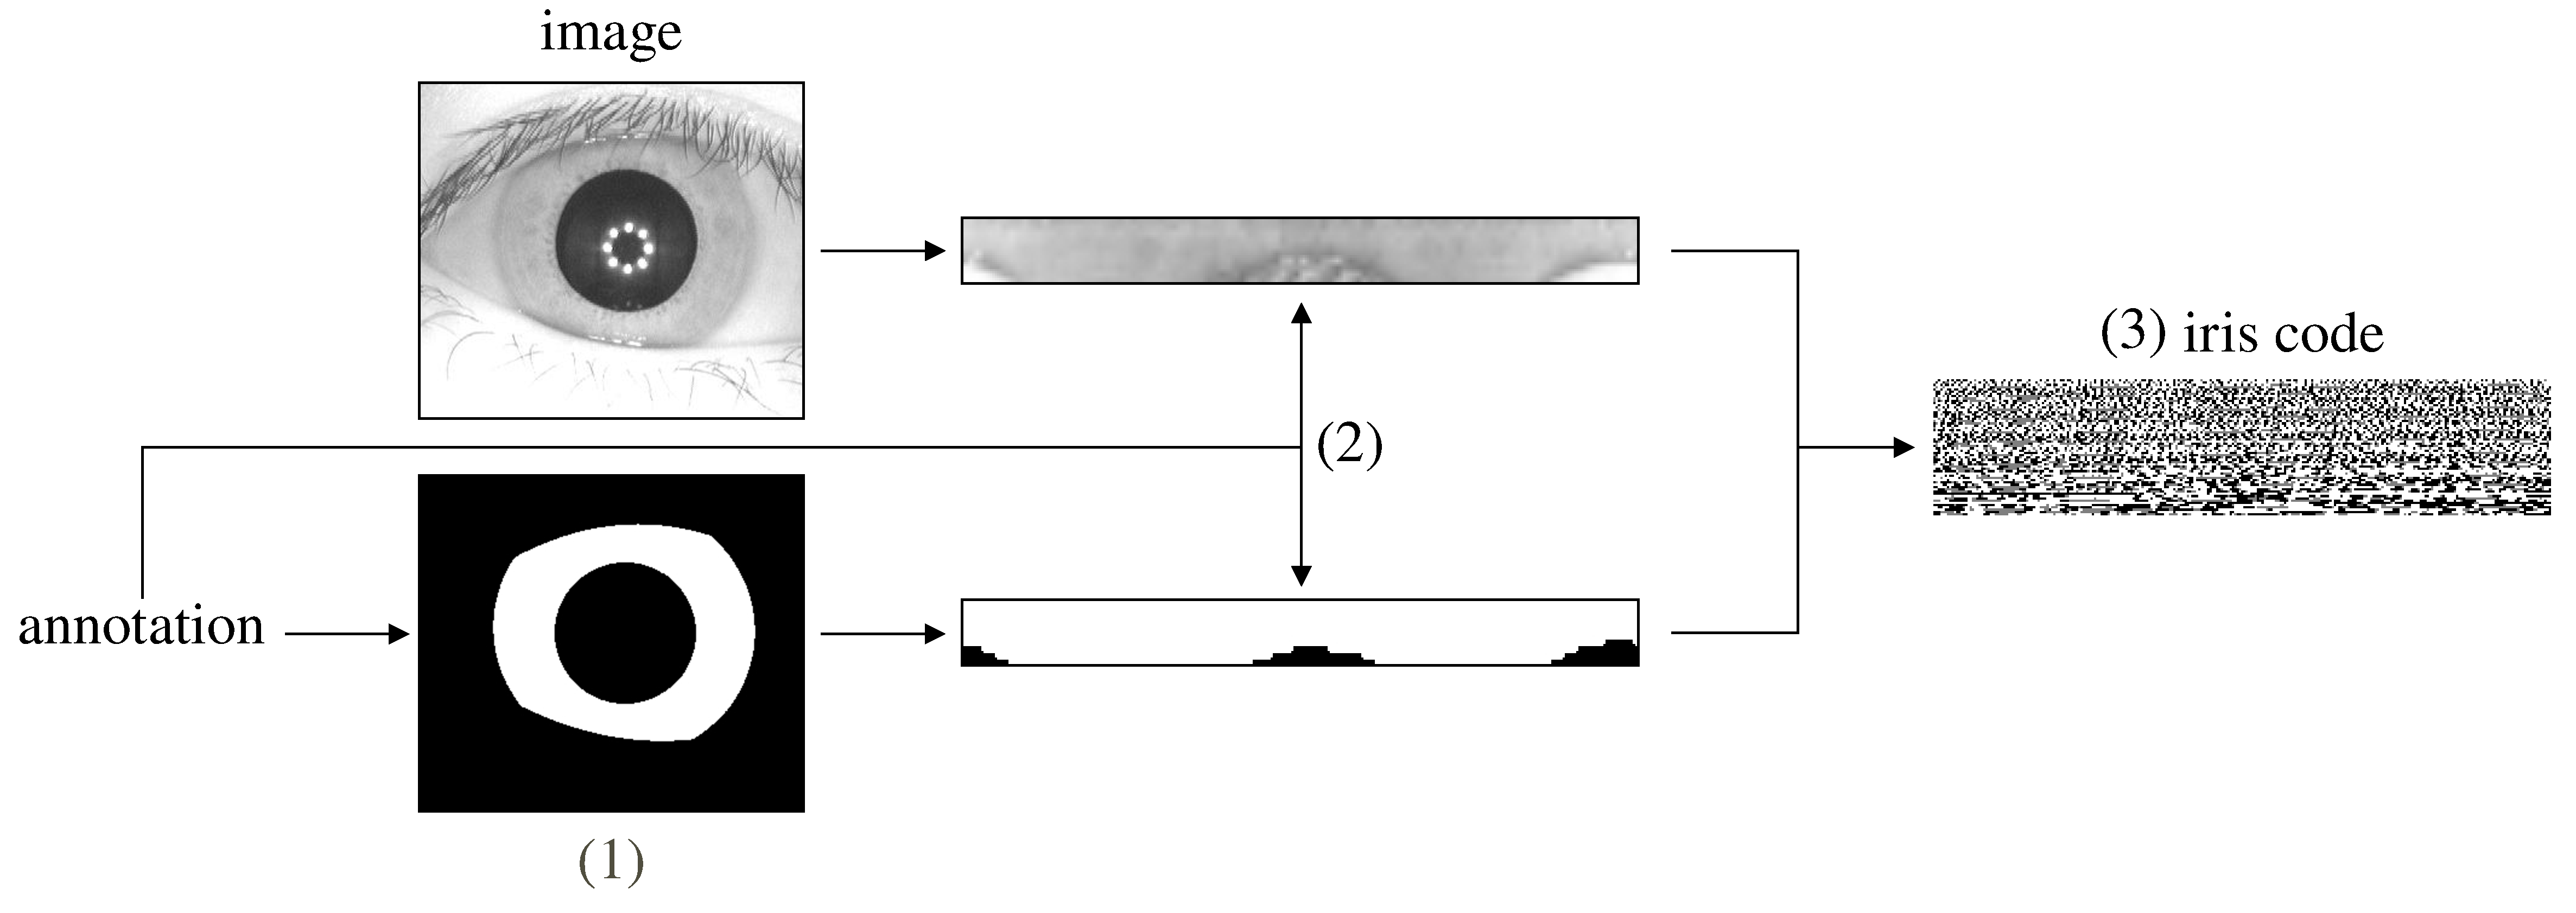
\includegraphics[width=1\linewidth]{figures/iris-code-gen.pdf}
    \caption{Iris code generation process. (1) The annotation (see text) is used to generate a binary mask of the visible parts of the iris. (2) The pupil and iris boundaries are used to create dimensionless polar projections of the iris and mask. (3) Gabor filters are applied to the polar image, quantized, and concatenated to a $16296$-element bit-vector which is the iris code. It is here visualised using black pixels for the value $0$ and white pixels for the value $1$. Pixels masked by the polar mask projection (and excluded from comparisons) are shown in grey (zooming might be necessary). }
    \label{fig:iris-code-gen}
\end{figure}

\section{Optimisation system}
Iris obfuscation has at least two objectives, one for the gaze accuracy and one for the iris recognition accuracy. This is problematic for classical optimisation where the goal is to find an extremum of a cost function with $\mathbb{R}$ as its domain. The field of multi-objective optimisation deals with exactly this kind of situation. A possible solution is to define a weighing of each sub-objective, i.e.
\begin{align}
	J^{\mathcal{O}}(I) = w_{gaze}J_{gaze}^{\mathcal{O}}(I) +  w_{iris}J_{iris}^{\mathcal{O}}(I),
\end{align}
as originally suggested by my supervisor in \cite{proposal}. This approach may be suitable when sufficient knowledge about the problem makes it possible to define reasonable values for the weights. It does, however, assume prior knowledge of the relative importance of the objectives. 

Instead, this thesis focuses on exploring the trade-offs between various objectives over a large range of possible parameter values for each obfuscation method. In the article this is done using grid-search due to the relatively limited search space. I also experimented with a population-based method for combining multiple objectives which preserves (something).\todo{what is something?}

\subsection{Pareto optimality}
A central idea in using these explorative methods is \textit{pareto optimality}. Pareto optimality is based on the concept that even when objectives are not comparable, it is possible to determine an ordering of the optimality of points. Figure (REF)\todo{figure} shows an example in two dimensions. The points marked in blue are objectively better than any of the black points. Being objectively better here means that it is at least as good in every dimension and better in at least one. This is called dominance - the full definition is shown in \cref{def:dominance}. Points that are not dominated by any other point is \textit{Pareto optimal} (\Cref{def:p-optimal}). The subset of all such points of a given set is called the \textit{Pareto frontier} (\Cref{def:p-frontier}). In this example, the blue points define the Pareto Frontier.

\begin{definition}[Dominance]\label{def:dominance}
Given points $\mathbf{x}$, $\mathbf{x'}$ and an objective function $f$ with domain $\mathbb{m}$, $\mathbf{x}$ dominates $\mathbf{x'}$ if and only if
\begin{align}
 \forall i \in \{1, \dots, m\} :&\quad f_i(\mathbf{x})\leq f_i(\mathbf{x'}) \\
and \quad \exists i \in \{1, \dots, m\} :&\quad f_i(\mathbf{x}) < f_i(\mathbf{x'}).
\end{align}
In other words $\mathbf{x}$ cannot be worse than $\mathbf{x'}$ for any objective and has to be better on at least one.
\end{definition}

\begin{definition}[Pareto optimal]\label{def:p-optimal}
A point $\mathbf{x}$ in set $S$ is Pareto optimal if
\begin{align}
    \nexists \mathbf{x'} \in S: \quad \mathbf{x'} \text{ dominates } \mathbf{x}.
\end{align}
\end{definition}

\begin{definition}[Pareto frontier]\label{def:p-frontier}
The subset of all Pareto optimal points in a given set.
\end{definition}

\subsection{In iris obfuscation}
For iris obfuscation, the Pareto frontier of the gaze metric (\cref{eq:ob_gaze}) and iris code similarity metric (\cref{eq:ob_iris}) defines the boundary between 



The optimisation goal used in the article (\cref{eq:obf-goal}) can be generalised to 
\begin{align}
	\begin{aligned}
    \max & J_{obf}(I, I^*)\\
    \min & \frac{J_{gaze}(I)}{J_{gaze}(I^*)},
\end{aligned}
\end{align}

for unconstrained optimisation. This is problematic since there is no relation valuing the relative importance of the two goals

\begin{figure}
    \centering
    \begin{tikzpicture}
    
    \draw[thick,->] (0,0) -- (4,0) node[anchor=north west] {x axis};
    \draw[thick,->] (0,0) -- (0,4) node[anchor=south east] {y axis};
    
    \draw [red] plot [smooth cycle] coordinates {(1,1) (1,3) (3,3) (3,1)};
    \end{tikzpicture}
    \caption{Caption}
    \label{fig:my_label}
\end{figure}



\section{Filtering approaches}
We approach the analysis of separating the iris signal and the gaze signal from a pragmatic perspective. An image may be visualised as a height-map to more clearly display the individual pixel values. 

\begin{figure}
	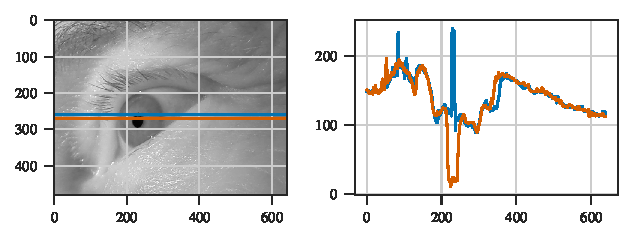
\includegraphics[width=1\textwidth]{figures/1dimage}
	\caption{Shows two one-dimensional slices of an eye-image to demonstrate how image intensity reveals the presence of the pupil and glint.}\label{fig:1dimage}
\end{figure}

\Cref{fig:1dimage} shows an eye image and a one-dimensional slice where the light intensity is graphed as a function of the x-position. Clearly, the portion covering the iris shows relatively chaotic changes but low variance compared to the rest of the image. The pupil-iris boundary and glint-pupil boundary which are used in our gaze-estimation method are clearly identifiable since they are represented as huge changes in intensity. These sorts of examples are typically also shown when introducing image edge detection, since it clearly demonstrates the connection between rate of change, i.e. the gradient, and the presence of an edge. 

When analysing the image as a Fourier series, two important factors stand out. Firstly, the iris seems to be dominated by a low-amplitude, very random signal. This indicates a range of small to medium wavelengths and high entropy. The edge regions, which are used by our gaze algorithm, instead look roughly like square waves. A square wave requires an infinite Fourier series to be represented accurately. Because the image is effectively band-limited, it is possible to recreate it with a finite series but it still spans the whole wavelength spectrum.

This signal analysis becomes important when considering methods for obfuscation. Our understanding of how the transformations affect different simpler signals may help us find suitable methods that are more well-suited to the application.

\todo{Should this be included somewhere?}
%\subsection{Measuring information in images}
%The term signal is rather abstract but is typically defined as a function that encodes or contains information of interest. Signals can be defined over temporal inputs, spatial inputs, or both. In the case of eye information processes, signals such as the captured eye images may be analysed individually as purely spatially divided signals or jointly as a time series of frames. The iris pattern in either its abstract or encoded form, is only resolved spatially while the gaze signal is usually analysed as a time-series. 




%When viewed as bandlimited discrete signals of two dimensions, images can be analysed structurally through the 

%To measure entropy and mutual information in images, it is necessary to formulate a method for defining the image in terms of a probability distribution. Specifically, it is necessary to define a model for the image distribution and estimate it using the image itself as data.

%The fundamental model is that each image can be represented by an unknown distribution $P_{img}$ of an unknown number of random variables $X^1, \dots, X^n$. A simple model is the intensity histogram which estimates a discrete distribution of intensity values assuming that each pixel is independent of each other. It can be defined as
%\begin{align}
%    P(I=i) = \sum_{x\in\mathcal{X}y\in\mathcal{Y}} \delta_{i, I_{x,y}},
%\end{align}
%where $\delta_{a, b}$ is the Dirac delta function. The downside to this approach is that no correlations between pixels are considered even though they clearly exist. For use in obfuscation measurement, this is problematic since the iris recognition methods use texture and not direct pixel intensities for detection. 

%In the most general terms, the distinct features of an iris pattern represents differences in the amplitude and phase of different frequencies. Many iris algorithms of the Daugman type use spatial phase responses to calculate a robust iris code. These traditional methods generally use some form of wavelet transform to separate spatial frequency-responses \parencite{daugman2007new}. %The convolutional neural-network based methods likely learn similar approaches as they have been shown to learn typical bandpass-filters like the wavelets used by Daugman (REF). 

%The image derivative, defined by its two partials, has excellent properties for measuring image texture complexity. The image derivative retains all information necessary to reconstruct the original image and is therefore still a valid upper bound on information measures. By defining $P_{img}$ as a joint distribution of the partial derivatives of the image
%\begin{align}
%    P(dx=i, dy=j) = \sum_{x\in\mathcal{X}y\in\mathcal{Y}} \delta_{i, {I_{\Delta x}}_{x,y}} \delta_{j, {I_{\Delta y}}_{x,y}},
%\end{align}

%Additionally, we also define joint distributions on convolutions with complex Gabor wavelets. A Gabor wavelet works as a bandpass filter, i.e. it responds only to certain frequency ranges. Defining a joint distribution over the Gabor response of a particular filter makes it possible to measure the entropy in certain frequency ranges which further... By definition however, a bandpass filter does not retain all the information in the original signal and can therefore not be used for definition of upper bounds.


